\section{Soil-Gas Spatial Variability And Preferential Pathways}

Preferential pathways can have a significant impact on spatial variability of contaminant vapors at a site.
This can manifest inside a house itself, as large concentration differences between rooms, as was the case due to a leaky bathroom plumbing fixture in the work by \citeauthor{pennell_sewer_2013}\cite{pennell_sewer_2013}; contaminant concentration was significantly higher in the upstairs bathroom than the basement, where higher concentrations are usually expected.
This was an example of yet a different preferential pathway effect than those modeled here, because it was associated with the failure of a trap on a sewer line.
Spatial variability in contaminant concentration can also manifest in the subsurface, which can be caused by a contaminant source\cite{chow_concentration_2007}, the building itself\cite{holton_creation_2018}, or as we will explore here - a subsurface preferential pathway.

\subsection{ASU House}

\citeauthor{guo_identification_2015}\cite{guo_identification_2015} explored the role that the ASU house land drain preferential pathway had on the spatial variability of contaminant vapors in the subsurface, and in particular in the gravel sub-base.
They used Kriging interpolation (discussed further below) to visualize the distribution of subsurface contaminant vapors using their collected subsurface contaminant vapor samples.
One snapshot of this work can be seen in Figure \ref{fig:guo_spatial_variability} where it clearly visible how the preferential pathway dramatically increased the contaminant vapor concentration in one half of the gravel sub-base layer - the half where the land drain preferential pathway exit was located.\par

\begin{figure}[htb!]
  \centering
  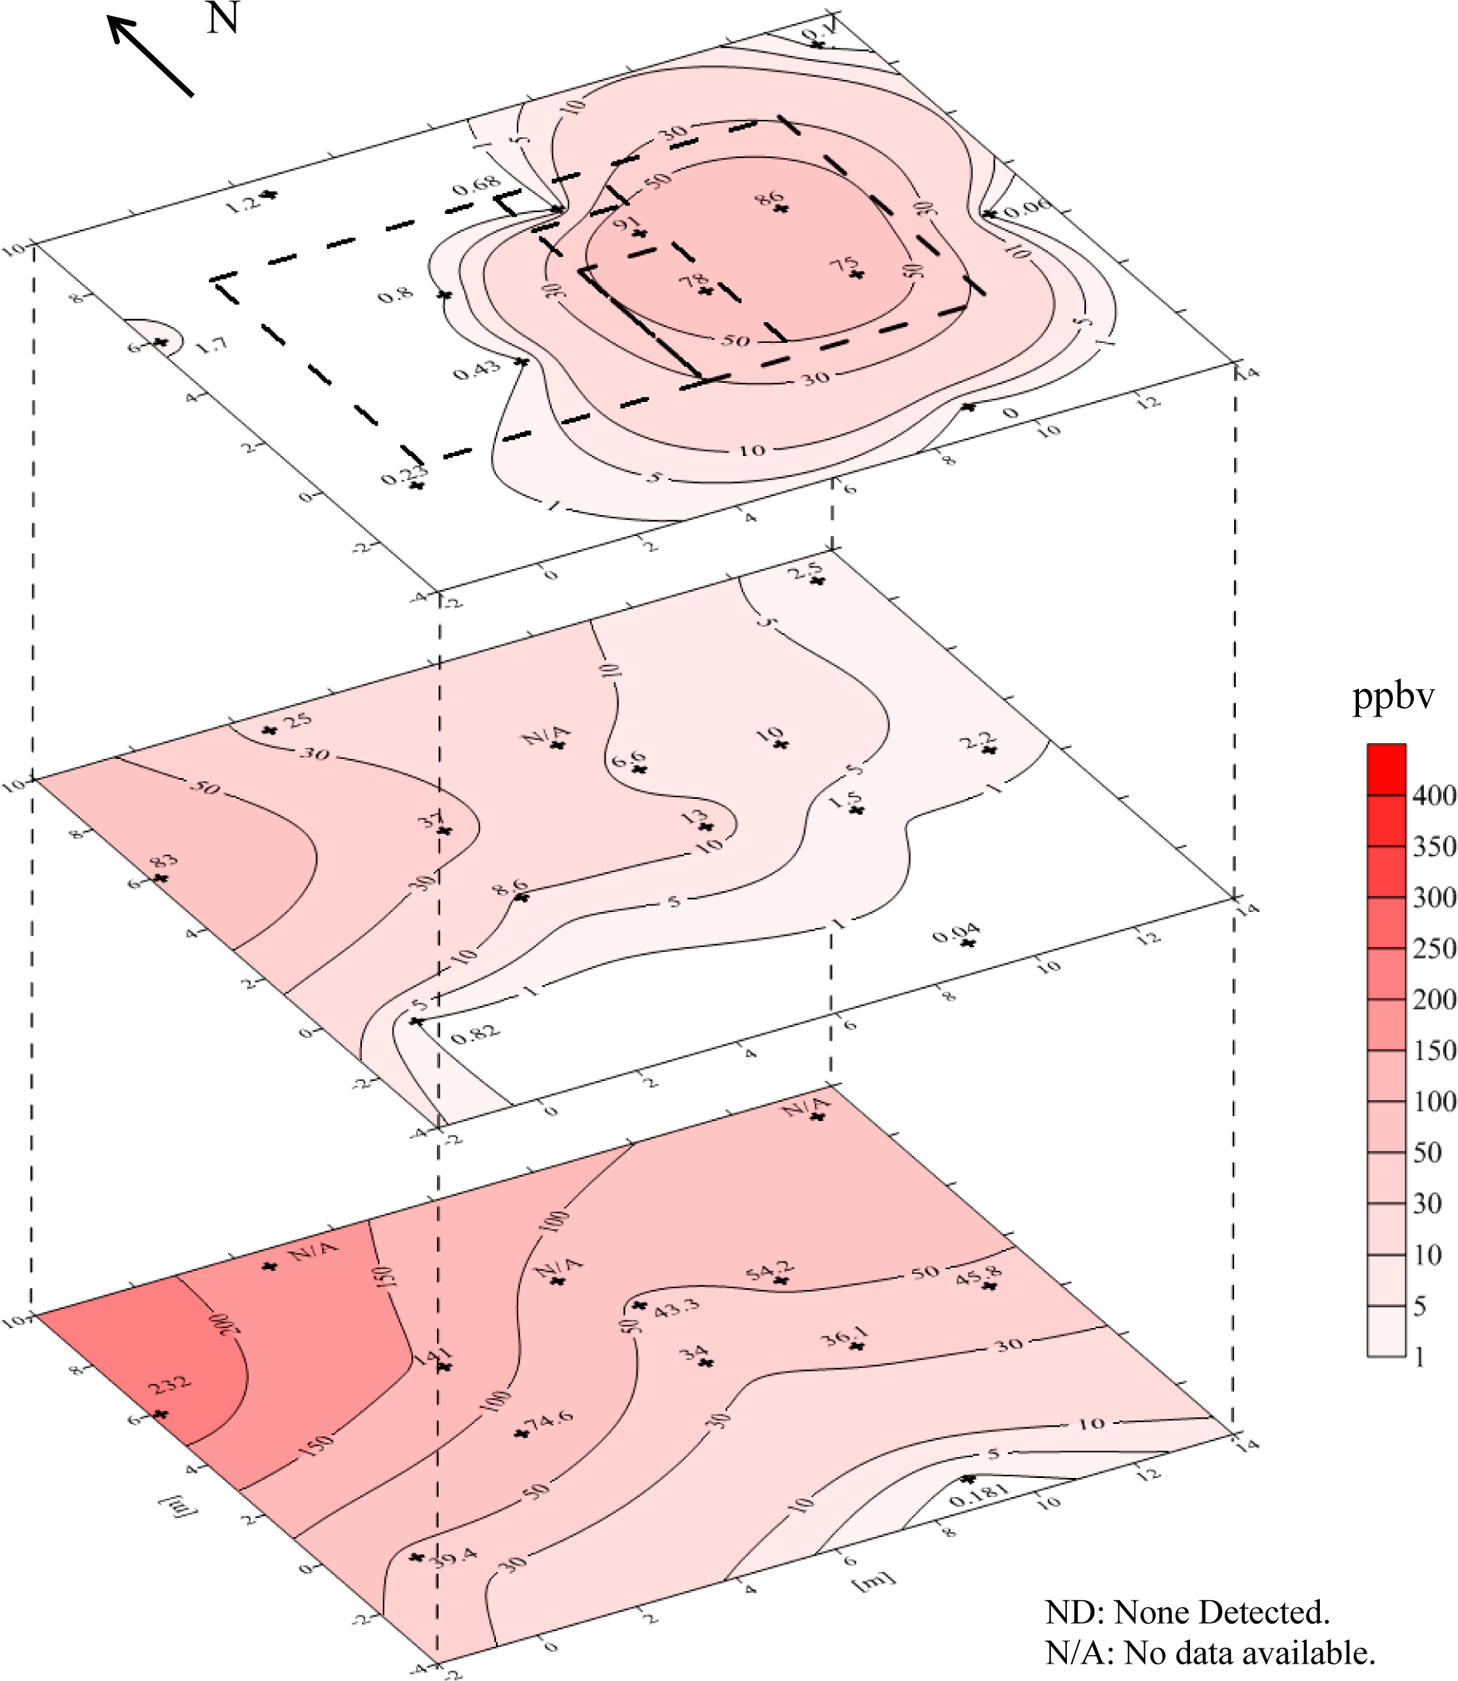
\includegraphics[width=0.85\textwidth]{guo_land_drain_spatial}
  \caption[Distribution of TCE contaminant vapors in the subsurface underneath the ASU house.]{Distribution of TCE contaminant vapors in the subsurface underneath the ASU house. The top layer is right beneath the foundation, with the two subsequent at \SI{0.9}{\metre} and \SI{1.8}{\metre} below the foundation slab. Snapshot from the period when the CPM system was active. Figure from \citeauthor{guo_identification_2015}\cite{guo_identification_2015}.}
  \label{fig:guo_spatial_variability}
\end{figure}

While this demonstrates the influence of a preferential pathway on subsurface spatial variability, it can be quantitively explored just how significant it can be.
To do this, we consider the attenuation from the sub-slab region to the indoor environment
\begin{equation}
  \alpha_\mathrm{subslab} = \frac{c_\mathrm{in}}{c_\mathrm{subslab,5}}
\end{equation}
using sub-slab vapor contaminant concentration data from location 5 of the ASU house (see Figure \ref{fig:land_drain_location}).
This was the sample location closest to exit of the land drain preferential pathway.
These data are visualized in a boxplot in Figure \ref{fig:asu_subslab_attenuation} where we consider the effects of CPM and the land drain preferential pathway on $\alpha_\mathrm{subslab}$.\par

\begin{figure}[htb!]
  \centering
  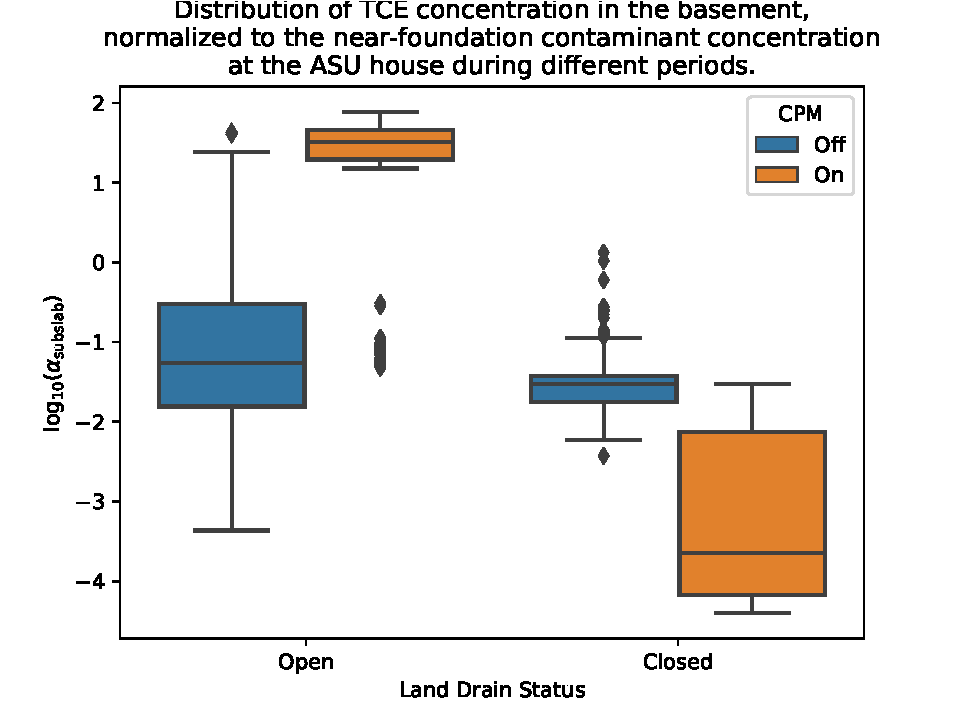
\includegraphics[width=0.85\textwidth]{asu_subslab_attenuation.pdf}
  \caption[Boxplot showing the distribution of $\alpha_\mathrm{subslab}$ considering the effects of CPM and the ASU house land drain preferential pathway.]{Boxplot showing the distribution of $\alpha_\mathrm{subslab}$ considering the effects of CPM and the ASU house land drain preferential pathway. Here $\alpha_\mathrm{subslab}$ is the attenuation from sub-slab sampling location 5 to the indoor environment. The box signifies the interquartile range (IQR) of values, with the central line representing the median value, and the top and bottom of the box are the 25th and 75th percentiles. The whiskers extend to 1.5 times the IQR. Markers indicate outlier data points that fall outside the whiskers.}
  \label{fig:asu_subslab_attenuation}
\end{figure}

Here we observe that when the preferential pathway was open and the CPM system active, $\alpha_\mathrm{subslab}$ usually exceeded unity by at least an order of magnitude, a situation that seemingly violates the expected concentration gradient from outside to indoors; we can likewise see that this is an observed occurrence when the preferential pathway was open but the CPM system inactive.
Normally, one would not expect $\alpha_\mathrm{subslab}$ to be even of the order of unity.
Examining the $\alpha_\mathrm{subslab}$ data from the period after the preferential pathway was closed, as well as $\alpha_\mathrm{subslab}$ data collected by the EPA in their VI database, $\alpha_\mathrm{subslab}$ would be expected to range from \num{1e-3} to \num{1e-1} with \num{3e-2} a commonly encountered value\cite{u.s._environmental_protection_agency_oswer_2015}.
In other words, the process of transport from subslab to indoor involves a substantial concentration gradient.
When $\alpha_\mathrm{subslab} \geq 1$ this can be an indicator that even though location 5 is only $~\SI{2}{\metre}$ away from the land drain preferential pathway exit, samples taken here may fail to capture the highest sub-slab contaminant concentrations; the highest contaminant vapor concentration in the subslab during the preferential pathway open period could  have been order of magnitude higher than recorded.
The complexity of the predicted $\alpha_\mathrm{subslab}$ that concentrations profiles in Figure \ref{fig:asu_subslab_attenuation} suggest that use of any single collected concentration value to characterize the whole subslab is very dangerous.\par

This highlights the large impact that a preferential pathway can have on subsurface spatial contaminant concentrations.
However, another possibility for explaining such high $\alpha_\mathrm{subslab}$ values is that they may indicate that there are some indoor contaminant sources present.
It was noted above that under certain circumstances, the flow of contaminant may reverse, and be in the direction from the house into the subslab.
This was not however the situation at the ASU house.
Nonetheless, this is another aspect of VI that investigators should be cognizant of high $\alpha_\mathrm{subslab}$ values (particularly those that are greater than unity) could indicate existence of an indoor source.
This is why during an actual in-house VI investigation, there is always a great effort made to identify any possible indoor sources of the contaminant of concern, and often these are found in consumer products which are removed before VI sampling takes place.\par

\subsection{EPA Duplex}

The spatial variability of the soil-gas contaminant concentration at the EPA duplex is investigated by interpolating the recorded data using the kriging technique.
Kriging is a commonly used technique in geostatistics where sparse spatial data can be interpolated over a larger spatial grid.
This interpolation is performed by calculating the spatial covariance between the known data points, making assumptions of spatial data distribution model - defining a kernel, and then fitting parameters to these kernels\cite{williams_prediction_1998}.\par

Here, the interest is in the situation at the EPA duplex, for which such analysis has not yet been performed.
The question to be answered is whether this analysis can shed more light on the temporal variability at that site- was a leaky preferential pathway injecting contaminant vapors into the soil adjacent the building?
Soil-gas contaminant concentration data were collected at multiple locations and at multiple depths around the duplex.
In Figure \ref{fig:indie_floorplan} we can see a number of ports labeled as SSP and SGP - these are the locations where soil-gas concentration data were collected.
Using the length scale in Figure \ref{fig:indie_floorplan}, approximate $x$ and $y$ coordinates for the location of each sampling port were extracted from the figure, and the bottom left corner of the figure is defined as $(x, y) = (0,0)$.
In the publicly available EPA duplex database\cite{noauthor_indianapolis_nodate}, the concentration of various contaminant at 5 different depths across time were recorded.
These together form a large dataset containing soil-gas contaminant concentration, their spatial coordinates in three dimensions as a function of time.\par

Kriging generally works best if the input data are normally distributed, which soil-gas contaminant concentration data generally not.
However, after a $\log_{10}$ transformation of the concentration data they generally normally distributed.
The kriging here was performed using the SciKit-learn Python package\cite{pedregosa_scikit-learn_2011}.
This requires input data, the data coordinates, a grid onto which data is to be interpolated onto, and a kernel.\par

A radial-basis function kernel, multiplied by a constant was chosen here, as it closely resembles the solution to the infinite domain diffusion equation.
\begin{equation}
  k(\vec{x}_i, \vec{x}_j) = C \exp{\Big( -\frac{1}{2} d\Big( \frac{\vec{x}_i}{l}, \frac{\vec{x}_j}{l} \Big) \Big)}
\end{equation}
$k$ is the kernel output value that determines the interpolated soil-gas concentration;
$\vec{x}_i, \vec{x}_j$ are the coordinates for some points $i$ and $j$;
$C$ is a constant that is determined by the software;
$d\Big( \frac{\vec{x}_i}{l}, \frac{\vec{x}_j}{l} \Big)$ is the distance between $\vec{x}_i$ and $\vec{x}_j$, scaled by a length parameters $l$, which is determined by the software.\par

The results of the kriging process are plotted using Plotly\cite{plotly_technologies_inc._collaborative_nodate} in Figure \ref{fig:kriging_results}.
It should be noted that these are soil-gas contaminant concentrations each from a period that is (by inspection) determined to be relatively "representative" of the overall temporally separated dataset.
In reality soil-gas contaminant concentrations fluctuate spatially in time, but there are some general trends that the analysis provides.\par

Figure \ref{fig:kriging_results} show how varied the soil-gas spatial variability for different contaminants can be.
In particular, we see that trichloroethene (TCE) here exhibit relatively minor spatial variability compared to chloroform or tetrachloroethene (PCE).
A likely explanation for this disparity is the role that the sewer played at this site.\par

In a later study of the EPA duplex, \citeauthor{mchugh_evidence_2017}\cite{mchugh_evidence_2017} found that PCE and chloroform could be found throughout the sewer network in the neighborhood; this was not true of TCE.
Looking again at PCE and chloroform in Figure \ref{fig:kriging_results}, we see that there is often a "hot spot" in the middle slice, approximately at a depth of \SI{-2.75}{\metre}, roughly in the middle of the front lawn area.
This is approximately the spot where the sewer line servicing the EPA duplex was located, which suggest that there was a leak in that vicinity.
The leak in that particular area, and thus the sewer preferential pathway at the site, is likely what significantly contributes to much the soil-gas contaminant concentration spatial variability.
This shows another way that a preferential pathways can the play a significant role at a VI site, and the importance of screening for them during a VI site investigation.\par

\begin{figure}[htb!]
  \centering
  % floorplan
  \begin{subfigure}{0.45\textwidth}
    \centering
    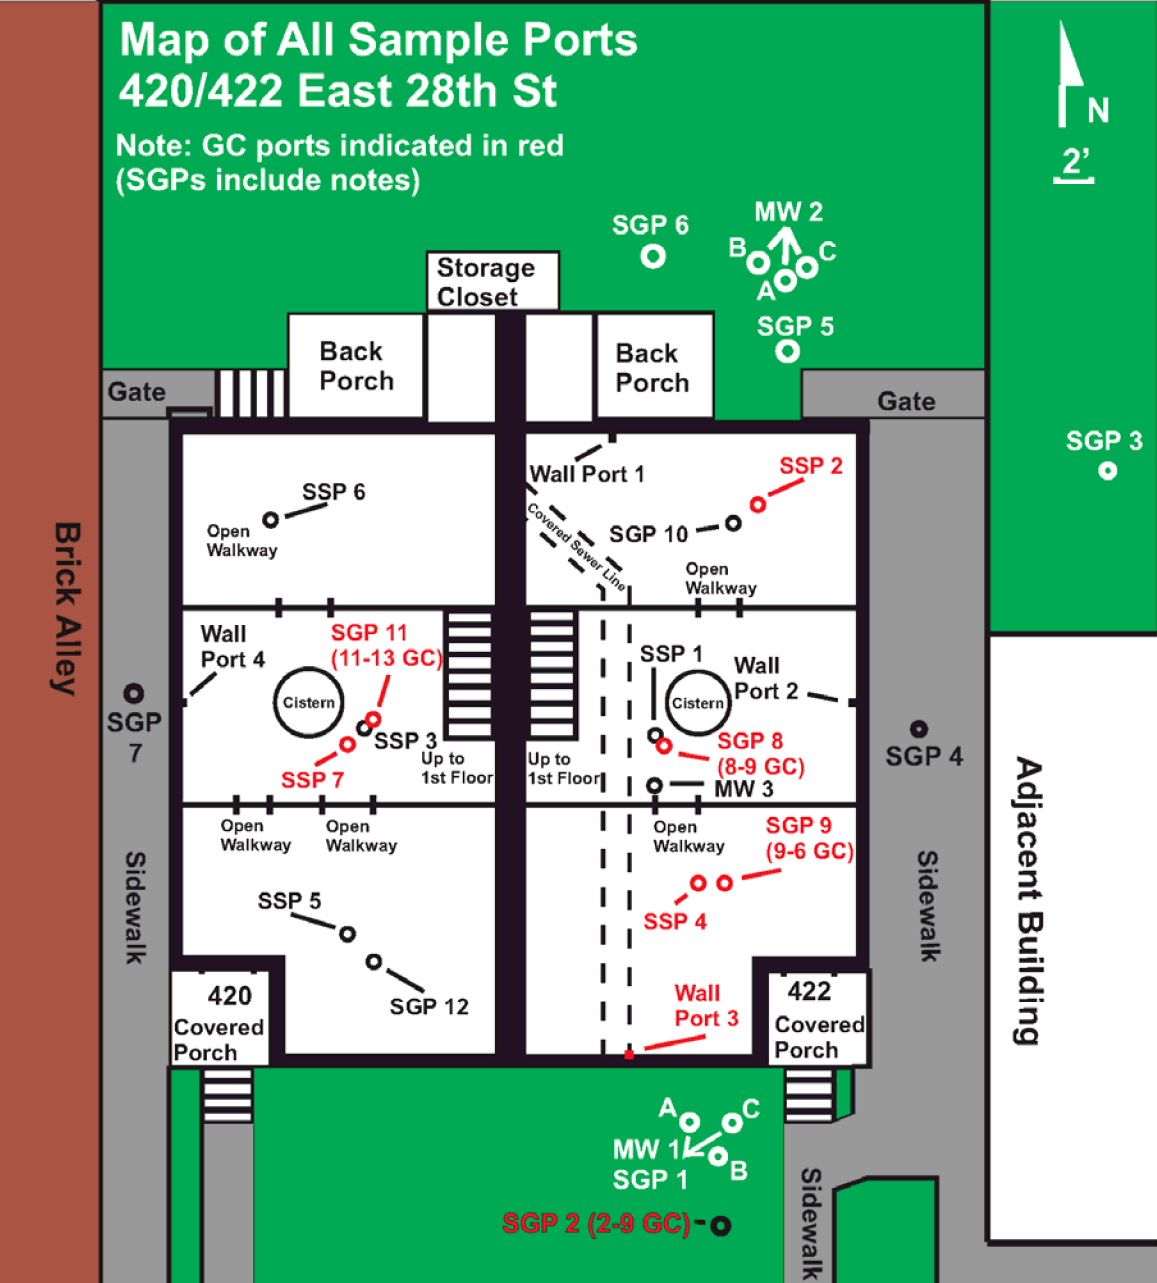
\includegraphics[width=0.75\textwidth]{indianapolis_floorplan.png}
    \caption{Floorplan of the EPA duplex. The soil-gas figures $x$ \& $y$ coordinates are relative to the bottom left corner.}
  \end{subfigure}
  % chlorform 2011-08-10
  \begin{subfigure}{0.49\textwidth}
    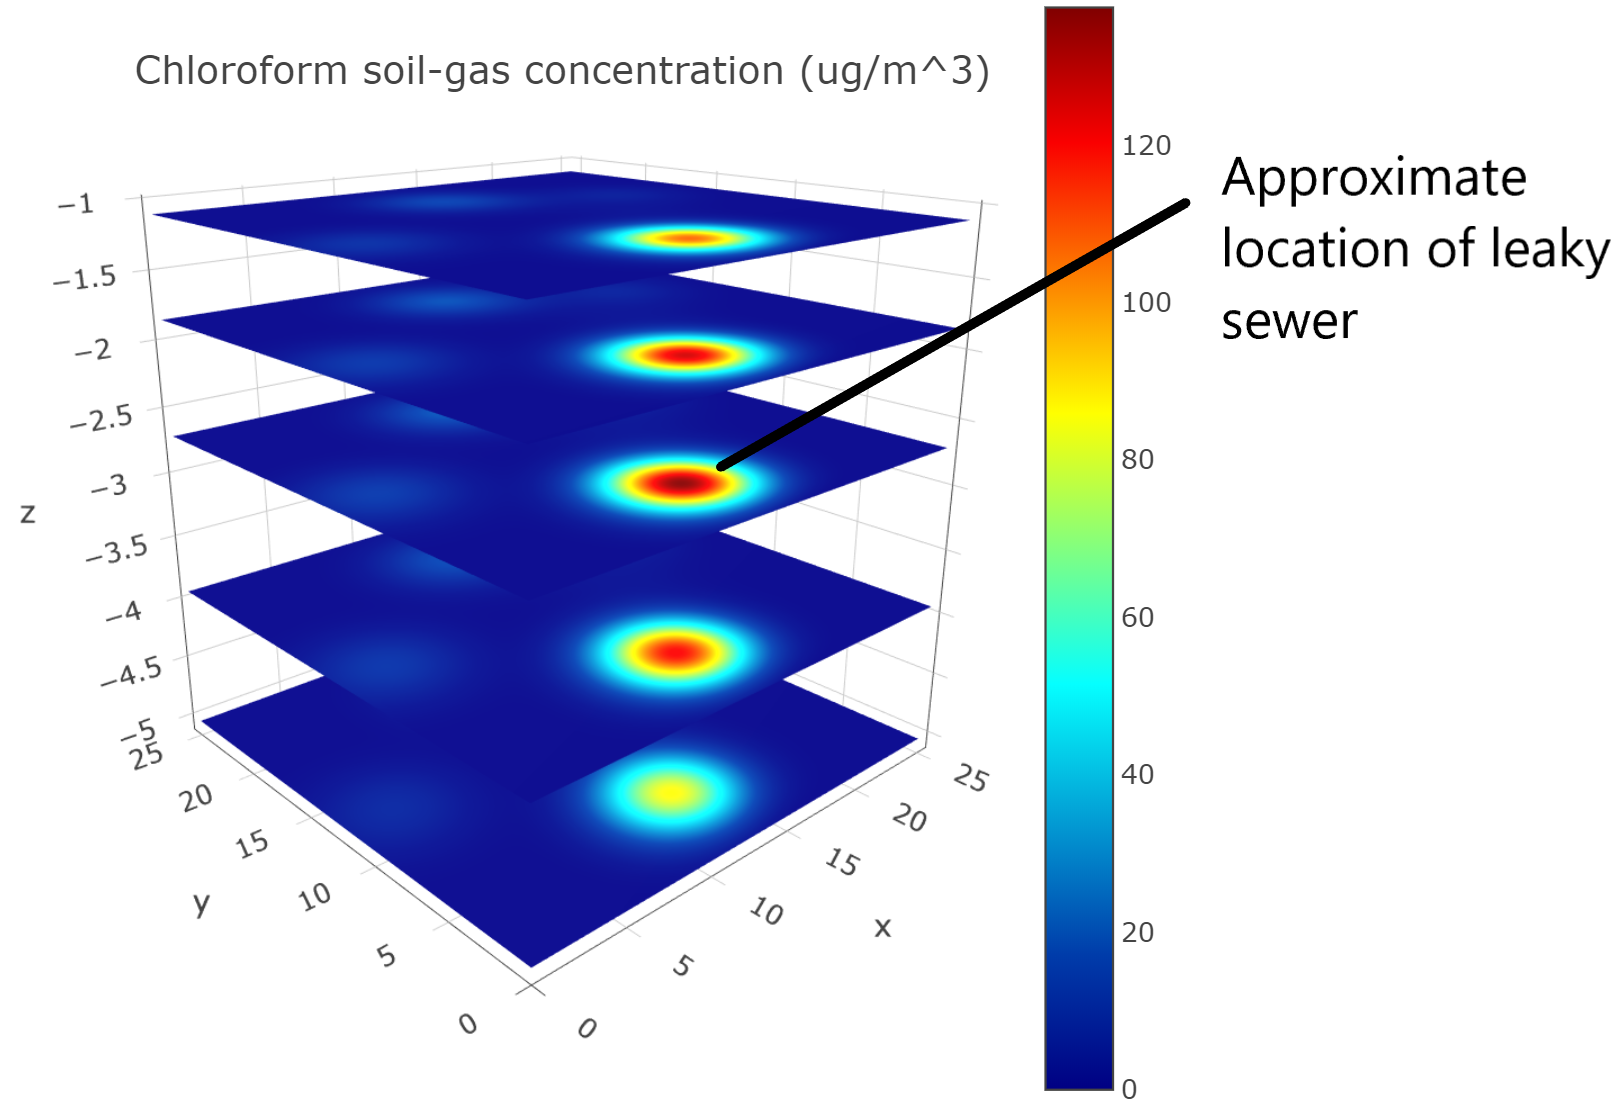
\includegraphics[width=\textwidth]{chloroform_epa_duplex.png}
    \caption{Soil-gas concentration of chloroform.}
  \end{subfigure}
  % tce 2011-06-01
  \begin{subfigure}{0.45\textwidth}
    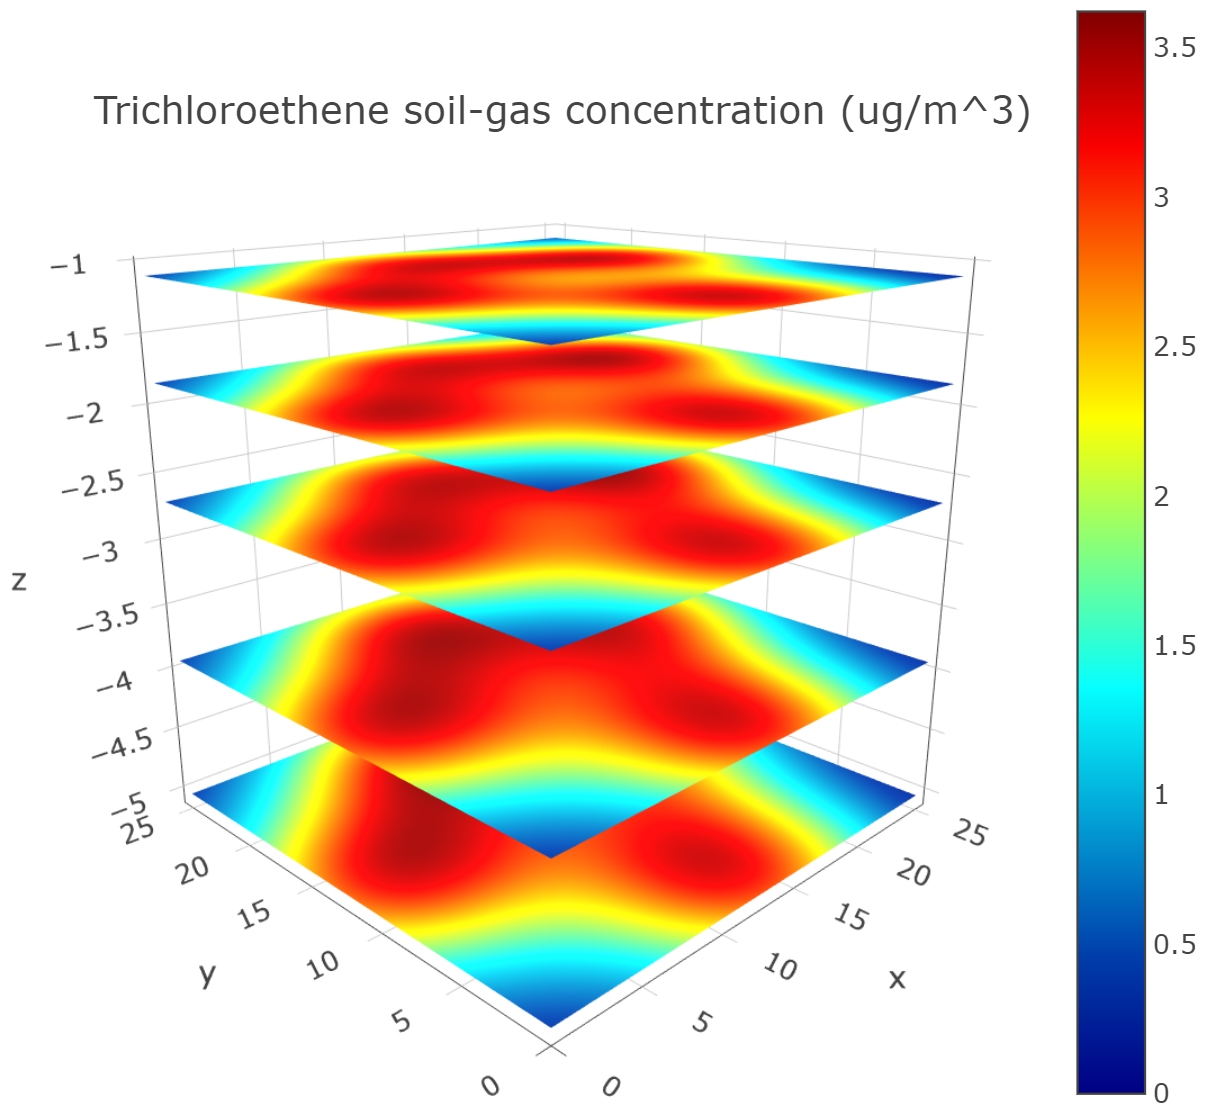
\includegraphics[width=\textwidth]{tce_epa_duplex.png}
    \caption{Soil-gas concentration of TCE.}
  \end{subfigure}
  % pce 2011-03-17
  \begin{subfigure}{0.45\textwidth}
    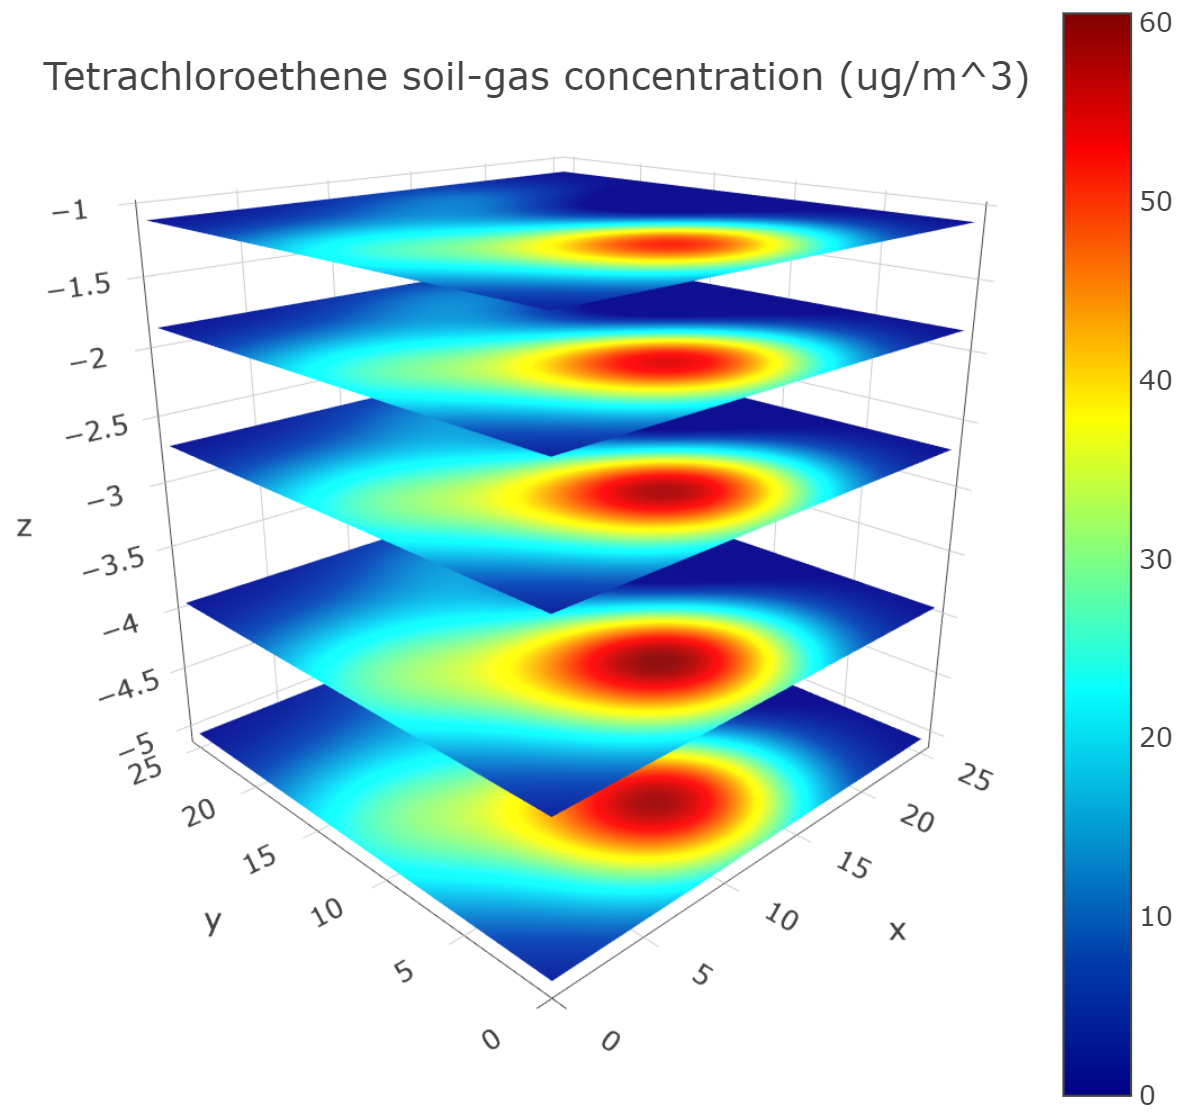
\includegraphics[width=\textwidth]{pce_epa_duplex.png}
    \caption{Soil-gas concentration of PCE.}
  \end{subfigure}
  \caption[Interpolated soil-gas contaminant concentrations for select contaminant underneath the EPA duplex.]{Interpolated soil-gas contaminant concentrations for select contaminant underneath the EPA duplex. Soil-gas concentrations profiles reveal a potential leak in the sewer line roughly underneath the EPA duplex front lawn.}
  \label{fig:kriging_results}
\end{figure}

Unfortunately, at this site, there were no data taken that would reveal the temporal variability of the PCE and chloroform concentrations in the sewer.
The kriging analysis merely gives some time-averaged pictures of the soil gas profiles adjacent to the house.
The study by \citeauthor{mchugh_evidence_2017}\cite{mchugh_evidence_2017} moreover offered a complicated picture of transport of these species in the sewer.
Thus, unlike the situation at the ASU House, it would be difficult to build a reliable model of the influence of this particular preferential pathway on the indoor air concentrations.
But what is clear is that in the presence of such a near-foundation source of contaminant vapors, the ordinary models of vapor transport from a groundwater source will also not apply.\par
